\subsubsection{Information}
\begin{itemize}
	\item \textbf{Course Name:} \href{https://www.coursera.org/learn/conduct-ux-research}{Conduct UX Research and Test Early Concepts}
	\item \textbf{Instructor:} \href{https://www.coursera.org/instructor/google-career-certificates}{Google Career Certificates}
	\item \textbf{Level:} Beginner
	\item \textbf{Enrolled on:} May 29, 2024
	\item \textbf{Finished on:} June 8, 2024
	\item \textbf{Grade Achieved:} 94.38\%
\end{itemize}

\subsubsection{Certificate}
\begin{flushleft}
	\begin{figure}[!ht]
		\centering
		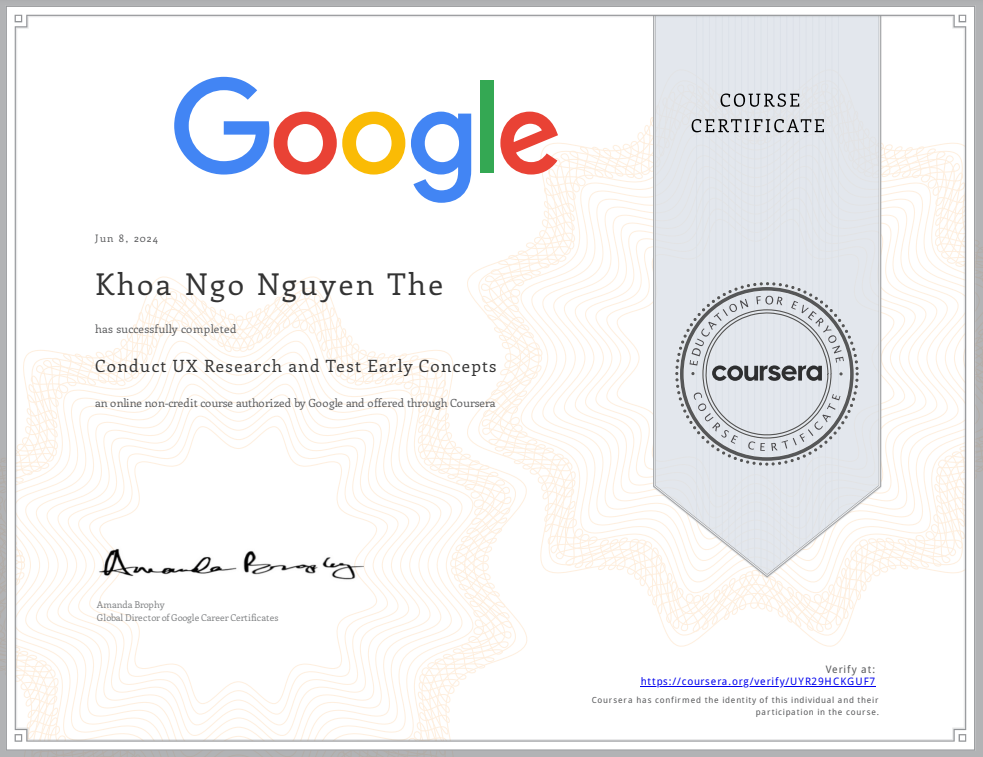
\includegraphics[width=0.85\textwidth]{imgs/Course4.png}
		\caption{Course 4 Certificate}
	\end{figure}

	Visit the online certificate for more info \href{https://www.coursera.org/account/accomplishments/verify/UYR29HCKGUF7}{here}
\end{flushleft}

\subsubsection{Summary}
\begin{flushleft}
	What I have learned after completing this course:
	\begin{itemize}
		\item Plan and conduct moderated and unmoderated usability studies.
		\item Synthesize observations from usability studies and come up with insights.
		\item Share research methodology and insights using persuasive presentation skills.
		\item Modify low-fidelity designs based on research insights.
	\end{itemize}
\end{flushleft}

\subsubsection{Details}
\begin{flushleft}
	\begin{description}
		\item[Module 1:] Planning UX research studies
		      \begin{itemize}
			      \item I have learnt how to plan a UX research study.
			      \item I have explored each of mentioned seven elements in detail, and I have created my own research plan to test the designs I developed in the previous course (Course 3).
			      \item I have also learnt how to respect user privacy and data when conducting UX research.
		      \end{itemize}
		\item[Module 2:] Conducting research with usability studies
		      \begin{itemize}
			      \item I have conducted a usability study, which is a research method that assesses how easy it is for participants to complete core tasks in a design.
			      \item I have also explored how to reduce bias and be inclusive when conducting usability studies.
			      \item I have taken notes while observing participants in a usability study.
		      \end{itemize}
		\item[Module 3:] Analyzing and synthesizing research results
		      \begin{itemize}
			      \item I have analyzed and synthesized all of the feedback from my research.
			      \item I have gathered data and observations in one place, organized the data using an affinity diagram, found themes, and come up with actionable insights.
		      \end{itemize}
		\item[Module 4:] Sharing research insights for better designs
		      \begin{itemize}
			      \item I have learnt techniques for presenting insights to various audiences, and improved my presentation skills to grab my audience's attention.
			      \item I have iterated on my designs, which means making revisions to create new-and-improved designs, based on insights from my research.
		      \end{itemize}
	\end{description}
\end{flushleft}